\section{Methods}\label{sec:Material and methods}

\subsection{Alloy Design Methodology}

\subsubsection{Design Space Definition and Compositional Constraints}

The design space is an 8-element HEA system, Al--V--Cr--Mn--Fe--Co--Ni--Cu, extending the 6-element Al--V--Cr--Fe--Co--Ni system investigated in Campaign~1~\cite{hastings2025accelerated} by the addition of Mn and Cu (rationale discussed in Section~1). The system includes all subsystems from 5 to 8 elements. Unlike Campaign~1, which imposed four constraints (single-phase FCC, density, thermal conductivity, and SFE regime), this study enforces only phase stability (i.e., single-phase FCC across the designated temperature range), adopting an open-ended strategy that avoids prematurely excluding regions of the composition space.

The initial compositional space is discretized at a resolution of 4 atomic percent, resulting in a pool of 3,365,848 unique compositions. To ensure manufacturability and focus on regions with potential for high performance, expert recommendations were used to impose upper limits on elemental fractions: Al $\leq 0.24$, V $\leq 0.24$, Cr $\leq 0.50$, Mn $\leq 0.40$, Fe $\leq 0.50$, Co $\leq 0.50$, Ni $\leq 0.60$, Cu $\leq 0.24$. These compositional bounds reduce the design space to 1,504,938 candidate alloys, of which 1,490,129 were successfully evaluated using CALPHAD due to solver limitations encountered on the high-performance computing cluster.

% \begin{figure*}[t]
%     \centering
%     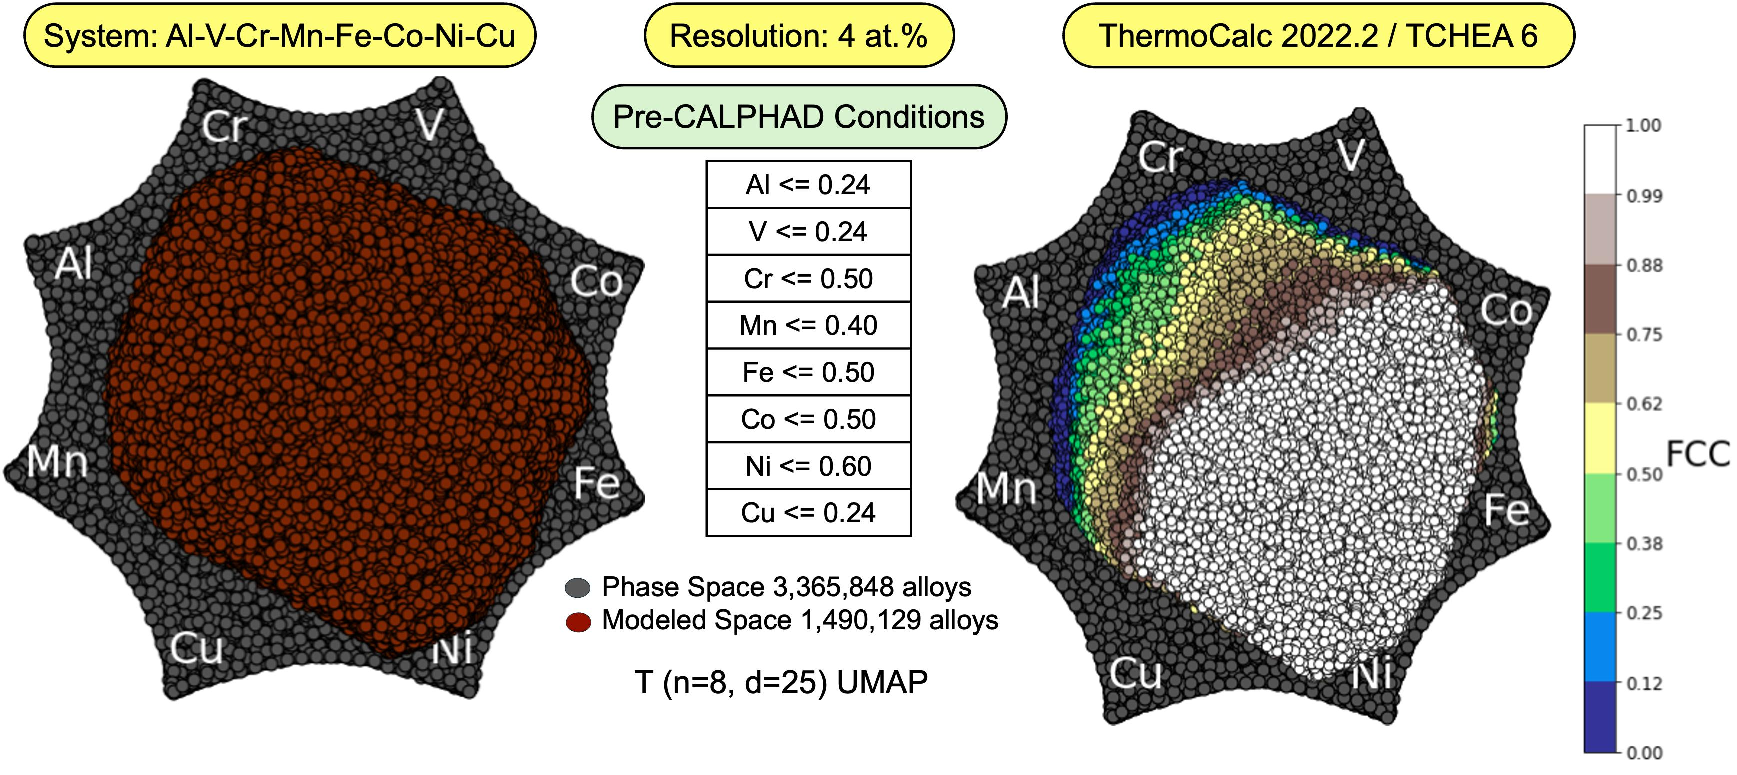
\includegraphics[width=0.8\textwidth]{Figures/feasible_space_v2.pdf}
%     \caption{
%     Visualization of the Al–V–Cr–Mn–Fe–Co–Ni–Cu compositional design space and feasible space for this study using UMAP dimensionality reduction.
%     \textbf{(Left)} The full 8-dimensional phase space sampled at 4\,at.\% resolution consists of 3,365,848 possible alloys (gray). \textbf{(Middle)} Expert-imposed compositional maximums, applied to filter for manufacturability, resulting in a reduced space of 1,504,938 alloys and a final modeled space of 1,490,129 alloys (brown).
%     \textbf{(Right)} Thermo-Calc (TCHEA6, 2022.2) predictions of FCC phase fraction at 700\textdegree{}C are mapped over the filtered space. Regions with FCC fraction $\geq$ 0.99 (white) define the feasible domain for Bayesian optimization.
%     This visualization highlights both the impact of practical compositional constraints and the nonuniform phase stability landscape across the HEA system.
%     }
%     \label{fig:umap_alloyspace}
% \end{figure*}


\subsubsection{Candidate Screening via CALculation of PHAse Diagram (CALPHAD) Predictions}

To enforce the FCC phase stability constraint, we screened the reduced compositional space using CALPHAD simulations. Thermo-Calc demonstrated effective single-phase predictions for the Al-V-Cr-Fe-Co-Ni system in Campaign~1~\cite{hastings2025accelerated}. Using the TCHEA6 database, we retained compositions with FCC phase fraction $\geq 0.99$ at 700$^\circ$C, reducing $\sim$3.36 million candidates to a feasible space of 26,621 alloys (approximately 0.8\% of the original design space). Visualizations of this downselection are included in the \textbf{SI}.

Phase prediction discrepancies in the first optimization iteration (BBB)---alloys predicted as single-phase FCC that experimentally formed sigma---motivated a reanalysis using the updated TCHEA7 database, released during this study. TCHEA7 enabled prediction of multiple phase regions (FCC, BCC, HCP, SIGMA, and liquid) across different temperature regimes. We reevaluated the design space at both 700$^\circ$C and 950$^\circ$C, advancing only alloys that retained FCC under both conditions. This dual-temperature screening yielded a final feasible set of approximately 27,240 candidate alloys.

\subsubsection{Sampling and Candidate Selection}

Given the large number of candidate alloys resulting from the initial filtering and screening (over 26,000), an efficient sampling strategy was critical to balance experimental feasibility with adequate coverage of the design space. For iteration BBA (zeroth iteration), sampling was performed over the initial TCHEA6-screened feasible space of 26,621 alloys (the TCHEA7 re-screening to 27,240 alloys occurred after iteration BBB). We implemented a hierarchical sampling strategy using k-medoids clustering. First, the entire feasible space was segmented based on chemical composition into 37 distinct subsystems, defined by the specific combination of elements present (for example, alloys containing all eight elements formed one subsystem, while seven-element alloys were grouped by which element is absent). Details of subsystem grouping are provided in \textbf{SI}.

Subsequently, we applied k-medoids clustering to the feasible space to extract a subset of 1000 representative alloys. In this clustering process, we enforced a constraint that at least one candidate alloy was selected from each of the 37 subsystems, with the number of selections per subsystem proportional to the number of feasible candidates available within that system. This approach guaranteed broad chemical coverage and preserved the diversity of the design space.

From this subset of 1000 alloys, a further down-selection identified 16 candidate alloys for synthesis. The downselection maximized representation across all 37 subsystems, ensuring that the final batch covered as many distinct chemistries as possible and provided a well-distributed initial training dataset for the Bayesian optimization loop.


\subsection{Synthesis}

The computationally designed alloys were synthesized using high-purity elemental ($>$ 99.9 wt.\%) precursors to produce $\sim$35~g dense, crack-free ingots using a Vacuum Arc Melting (VAM) (Edmund B\"{u}hler AM 200) system. The elements were initially melted in Cu crucibles under a high-purity Ar atmosphere. Each ingot was flipped and re-melted 10 times to promote overall uniform chemical homogeneity. Mass loss was monitored throughout processing, and ingots showing losses greater than 0.5\% were reprocessed. Post-solidification, the ingots were homogenized between 950$^\circ$C to 1150$^\circ$C temperature ranges for 24~h in a Centorr LF Series Model~22 high-temperature furnace. The homogenization heat treatment temperatures were selected based on the predicted solidus temperature. Prior to heating, the furnace chamber was purged with Ar gas multiple times to achieve a vacuum of $\sim$5~$\times$~10$^{-5}$~torr. The heat treatment was conducted under a low-pressure Ar atmosphere ($<$10$^{-2}$~torr), followed by furnace cooling.

The homogenized ingots were subsequently cold rolled to a $\sim$60\% reduction in thickness. For recrystallization, the rolled specimens were wrapped in stainless-steel foil with Ti sponge sacrificial getter to minimize oxidation. Recrystallization was performed at 950\textdegree C for 30~min, followed by water quenching to suppress secondary-phase precipitation during cooling.

Test sample profiles were precision-cut using wire-Electrical Discharge Machining (EDM). Approximately 4 miniaturized flat tensile specimens, modeled following modified SS-3 designs, were prepared for quasistatic tension testing. Each tensile specimen had a total length of $\sim$26~mm, a gauge length of $\sim$8~mm, and a typical cross-sectional area of 3~$\times$~1~mm$^{2}$, with the loading axis aligned parallel to the rolling direction. Prior to testing, the tensile samples were ground using 120~grit SiC abrasive papers to ensure grip section parallelism, and pinholes were drilled using carbide drill bits. Additional specimens were prepared for microstructural and mechanical characterization, as follows: two specimens, each $\sim$2~mm thick with an exposed face area of 8.4~mm$^{2}$ normal to the long rolling direction, were designated for nanoindentation. Another two samples, 1.2~mm thick with a face area of 14.4~mm$^{2}$ (also normal to the rolling direction), were allocated for scanning electron microscopy (SEM), electron backscatter diffraction (EBSD), energy-dispersive X-ray spectroscopy (EDS), X-ray diffraction (XRD), and Vickers hardness (HV) measurements. A schematic of the specimen geometries is shown in \autoref{fig:Sample Cutting Protocol}.

\begin{figure}[t]
    \centering
    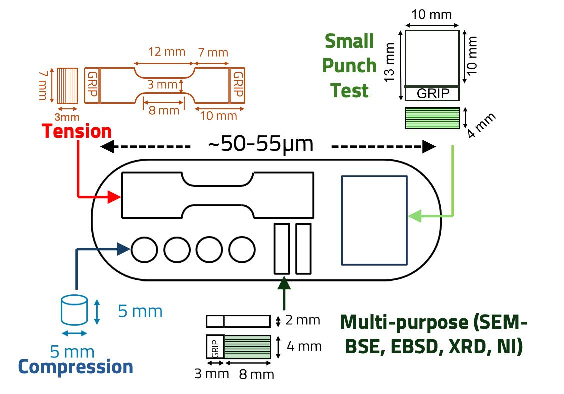
\includegraphics[width=0.9\columnwidth]{Figures/Cutting_Schematic_C2.pdf}
    \caption{Representative schematics of ingots post-cold rolling with corresponding approximate sample dimensions for distinct characterization tasks: SEM/EBSD, EDS, XRD, and mechanical (Vickers, Nanoindentation) analyses, quasistatic tensile deformation, and Kolsky-bar compression dynamic mechanical response tests.}
    \label{fig:Sample Cutting Protocol}
\end{figure}

We note that manganese contents exceeding 20 atomic percent introduced significant challenges during arc melting. Mn has a relatively low boiling point and high vapor pressure compared to the other constituent elements, making it volatile under the localized temperatures generated during arc melting. This volatility leads to Mn evaporation, resulting in deviations from the nominal composition and causing microstructural inhomogeneities and porosity in the cast ingots. Mn loss disrupts the stability of the intended single-phase FCC structure and promotes the formation of intermetallic compounds or segregated phases.


\subsection{Verification}

\subsubsection{Metallography}

Microstructural characterization and nanoindentation samples were prepared by mechanical polishing using a Buehler AutoMet 250 autopolisher with diamond suspensions down to 1~$\mu$m, followed by vibratory polishing in 0.04~$\mu$m colloidal silica for EBSD analysis. A high-throughput sample preparation workflow was developed over the course of the campaign, evolving from individual mounting (8 samples per batch) to large-format aluminum platens supporting 16 or more samples simultaneously, with laser marking for traceability. Details of this workflow evolution are provided in the \textbf{SI}.


\subsubsection{Chemical, Microstructural, and Phase Analyses}

Compositional analysis was performed using a Tescan FERA-3 Model GMH Focused Ion Beam Microscope equipped with an Oxford energy-dispersive X-ray spectroscopy (EDS) detector, operated at an accelerating voltage of 20 kV. EDS point measurements were obtained from three spatially distinct regions of each processed ingot, with five acquisition points per region and an integrated time of $\sim$50~s per point. The overall composition of each ingot was determined as the arithmetic mean of the 15 measurements. Inter-regional variability was evaluated to assess chemical homogeneity. Representative EDS results from three independent synthesis iterations are presented in \autoref{fig:EDS}. The mean deviation between measured and nominal compositions was $\sim$0.42~at.\%, with 99\% of individual elemental measurements deviating by less than 1~at.\%, confirming compositional uniformity across all synthesis batches.

\begin{figure}[t]
    \centering
    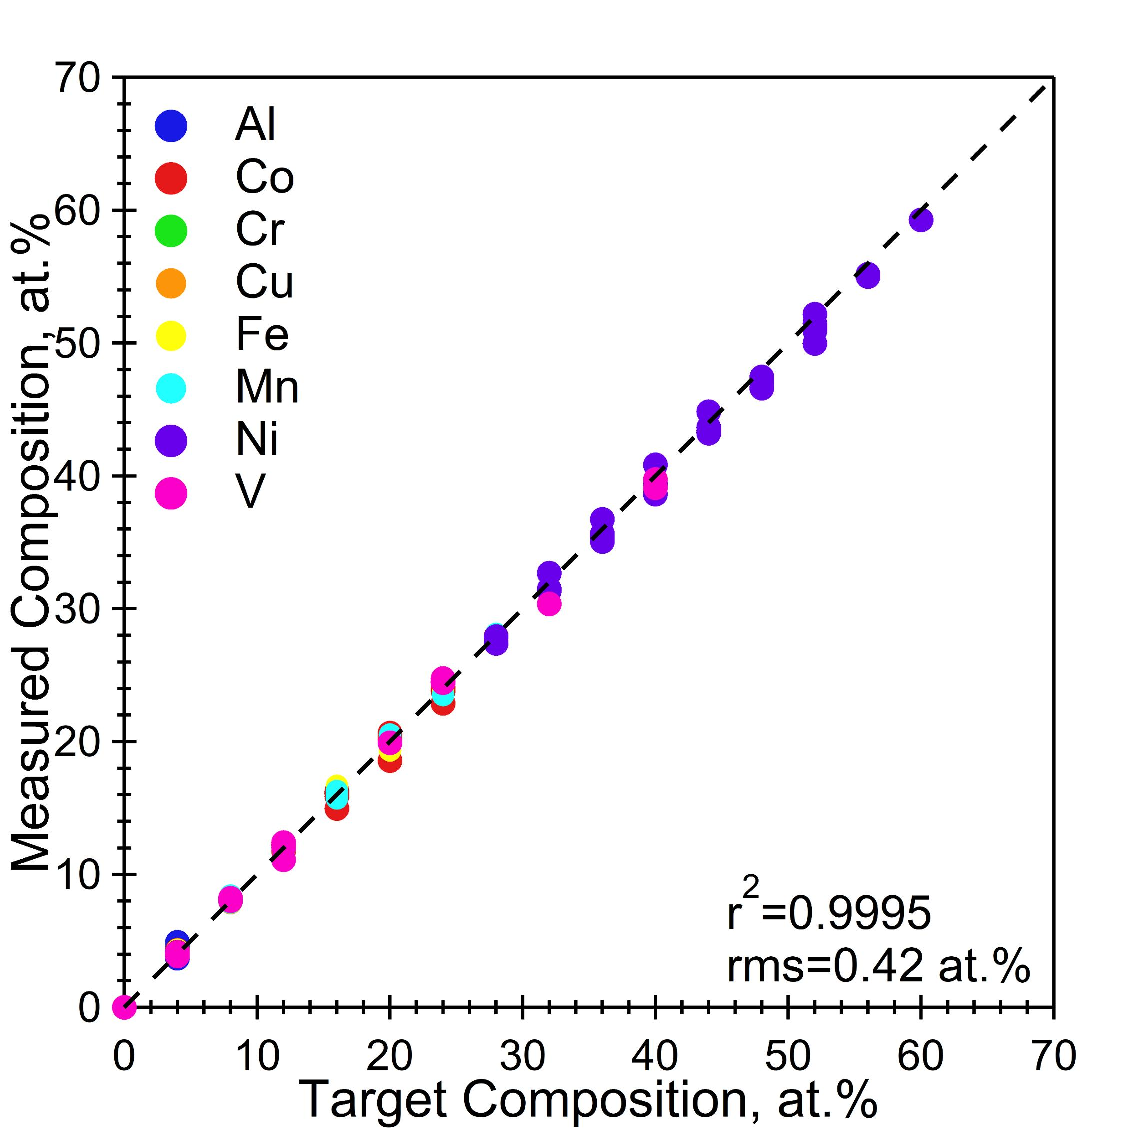
\includegraphics[width=0.9\columnwidth]{Figures/eds_summary.pdf}
    \caption{Comparison between target and realized chemistry for the samples generated in this study.}
    \label{fig:EDS}
\end{figure}

Microstructural characterization of the undeformed samples was performed by backscattered electron (BSE) imaging at 15~kV using a Phenom XL scanning electron microscope (SEM) with a working distance of $\sim$6~mm. Electron backscatter diffraction (EBSD) measurements were carried out using a FERA SEM equipped with an Oxford Symmetry CMOS-based EBSD detector, operated at an accelerating voltage of 20~kV, a beam current of 18~nA, and a specimen tilt angle of 70$^\circ$. Crystallographic orientation (IPF) maps were acquired on surfaces normal to the cold-rolling direction over an area of approximately 1~$\times$~1~mm$^{2}$, using a step size of $\sim$2~$\mu$m.

Room-temperature X-ray diffraction (XRD) measurements were conducted using a Bruker D8 Discover diffractometer with Cu K-$\alpha$ radiation ($\lambda$ = 1.5406~\AA) and a 1~mm aperture collimator. Diffraction patterns were collected using a Vantec 500 area detector over a 2$\theta$ range of 30--80$^\circ$. Phase identification and diffraction pattern analysis were performed using the MAUD software package.

\subsection{Characterization}

The optimization targets five objectives that together span the quasi-static--to--dynamic response space: (a)~yield strength (YS), (b)~the UTS/YS ratio (a proxy for strain hardening capacity and resistance to strain localization), and (c)~engineering strain at UTS (ductility reserve before peak load), all three extracted from uniaxial tensile tests; (d)~the dynamic-to-quasi-static hardness ratio ($H_\text{dyn}/H_\text{qs}$), obtained from nanoindentation and SHPB measurements, which quantifies how much the alloy strengthens under impact loading; and (e)~depth of penetration (DoP), computed from finite-element ballistic simulations calibrated to the tensile and SHPB data acquired within the same iteration---the only objective derived from simulation rather than direct measurement. Campaign~1 used hardness as an objective; here we replace it with the tensile-derived metrics, which connect more directly to bulk deformation behavior and are less sensitive to local microstructural heterogeneity.

\subsubsection{Quasistatic Tensile Deformation}

Uniaxial tensile tests were conducted at ambient temperature using an MTS 810 servo-hydraulic testing system equipped with an 11.12~kN (2500~lbf) load cell, under a constant quasi-static strain rate of 5~$\times$~10$^{-4}$~s$^{-1}$. Axial strain was measured using an MTS clip-on extensometer mounted directly on the specimen gauge section. An initial force-controlled loading sequence was performed to verify specimen alignment, modulus consistency, and linearity of the elastic response. At least 2 tests were conducted for each condition to ensure reproducibility. Tensile tests were terminated upon complete fracture. True stress--strain ($\sigma$--$\varepsilon$) curves were calculated, from which the ultimate tensile strength (UTS), 0.2\% offset yield strength (YS), and uniform elongation ($\varepsilon$) were determined.

\subsubsection{Nanoindentation}

% Each sample was indented using a KLA Instruments iMicro nanoindenter fitted with a Berkovich diamond tip. Hardness ($H$) and reduced modulus ($E_r$) were determined following the Oliver and Pharr method \cite{Oliver1992}.

% Strain rate jump tests were conducted to assess rate-dependent mechanical behavior across all candidate alloys. Automated methods for quantifying projected contact areas and correcting for pile-up effects were developed to improve measurement precision and throughput; details of the automation pipeline are provided in the \textbf{SI}. The strain rate sensitivities obtained from nanoindentation were cross-validated against SHPB results and found to be in close agreement, typically within one standard deviation.

Each sample was indented using a KLA Instruments iMicro nanoindenter fitted with a Berkovich diamond tip. Hardness ($H$) and reduced modulus ($E_r$) were determined following the Oliver and Pharr method \cite{Oliver1992}. Conventional nanoindentation hardness values were obtained from strain-rate jump tests using a constant $\dot{P}\!/P$ protocol, with hardness reported at an indentation depth of \SI{2000}{\nano\meter}. A minimum of 10 strain-rate jump indents was performed for each alloy. Indents were typically spaced \SI{100}{\micro\meter} apart to prevent overlap between neighboring plastic zones.
Strain-rate jump tests were conducted to assess rate-dependent mechanical behavior across the candidate alloys. These measurements were used to estimate indentation strain-rate sensitivity. The strain-rate sensitivities obtained from nanoindentation were cross-validated against SHPB results and were found to be in close agreement, typically within one standard deviation.
Projected contact areas were corrected for pile-up for each individual indent. The projected contact area was calculated from the calibrated tip area function, $A(h_c)$, determined from fused silica calibration \cite{Oliver1992}, and evaluated at the contact depth, $h_c$. The contact depth was calculated from the measured indentation depth, h, using an experimentally measured pile-up ratio,
\[
\eta = \frac{h_c}{h}
\]

The pile-up ratio was measured after each indentation using optical profilometry. First, the nominal indentation area, $A_N$, was determined from the region below the original sample surface. This area scales with $h^2$. The actual residual contact area, $A_R$, was then segmented using a gradient-based method that identifies the Berkovich impression boundary; this area scales with $h_c^2$. Assuming self-similar Berkovich geometry, the pile-up ratio was calculated as
\[
\eta = \frac{h_c}{h} \approx \sqrt{\frac{A_R}{A_N}}
\]

An independent value of $\eta$ was measured for every indent and applied to the corresponding hardness and modulus calculation. This correction was applied to strain-rate jump, quasistatic, and dynamic hardness measurements. The pile-up correction typically reduced the measured hardness by approximately 5 to 15\%, depending on alloy composition and testing condition. Custom analysis scripts were developed to extract the instrument data and automate projected contact area quantification; additional details of the image-analysis workflow are provided in the SI.



\subsubsection{High Strain Rate Nanoindentation}


% A nanoindentation instrument was adapted for impact testing at strain rates exceeding $10^{3}~\text{s}^{-1}$. Nanoindentation impact tests were conducted using an indenter system containing a hexapod specimen stage and an InForce 1000 actuator customized to measure displacements at high acquisition rates using a Michelson interferometer; full details of this setup can be found in \cite{Hackett2023}. All tests were performed with a Berkovich three sided pyramid tip.

% Quasistatic constant indentation strain rate tests were conducted using a constant $\dot{P}/P$ protocol (force rate over force) with a target $\dot{P}/P = 0.2~\text{s}^{-1}$ and a target load of 1~N. Dynamic tests consisted of indentation impact tests with an impact force of 20~mN, followed by re-loading at the same indent location up to 1~N at a target $\dot{P}/P = 0.2~\text{s}^{-1}$. The reloading step was included to enable comparison of the dynamic-to-quasistatic hardness ratio, $H_{\text{DYN}}/H_{\text{QS}}$, obtained from separate tests with that obtained from a single testing point; the results of this comparison will be presented in a separate study.

% Hardness was evaluated at an indentation depth of 2000~nm by dividing the load at that depth by the expected projected contact area. The projected contact area was calculated from the tip area function, $A(h)$, determined through a separate calibration procedure on fused silica \cite{Oliver1992}, and evaluated at the contact depth, $h_c$. The contact depth was obtained by multiplying the indentation depth by the contact-depth-to-indentation-depth ratio, $h_c/h$. This ratio was determined experimentally by imaging each indentation impression after testing using a laser confocal microscope. The residual contact area, $A_R$, was measured by manually tracing the impression boundary, and the nominal contact area, $A_N$, was obtained by thresholding the images. The ratio was then estimated as:
% \begin{equation}
% \frac{h_c}{h} = \sqrt{\frac{A_R}{A_N}}.
% \label{eq:contact_depth_ratio}
% \end{equation}

High strain rate nanoindentation was performed on a separate custom instrument adapted for indentation impact testing at strain rates exceeding $10^{3}\ \mathrm{s^{-1}}$. The instrument includes a hexapod specimen stage and an InForce 1000 actuator customized to measure displacements at high acquisition rates using a Michelson interferometer; full details of this setup are provided by Hackett \etal\ (2023). All tests were performed with a Berkovich three-sided pyramidal diamond tip.

The high strain rate instrument was used to measure the dynamic-to-quasistatic hardness ratio, $H_{\mathrm{DYN}}/H_{\mathrm{QS}}$, which was incorporated into the Bayesian optimization loop. Dynamic hardness, $H_{\mathrm{DYN}}$, was measured from indentation impact tests with an effective $\dot{P}/P = 2 \times 10^{3}\ \mathrm{s^{-1}}$. Quasistatic hardness, $H_{\mathrm{QS}}$, was measured on the same instrument using a constant $\dot{P}/P = 2 \times 10^{-1}\ \mathrm{s^{-1}}$. A minimum of 10 dynamic impact indents and 10 quasistatic indents was performed for each alloy, with indents typically spaced $100\ \mu\mathrm{m}$ apart.

Dynamic tests used an impact force of $20\ \mathrm{mN}$, followed by reloading at the same indentation location to $1\ \mathrm{N}$ at $\dot{P}/P = 2 \times 10^{-1}\ \mathrm{s^{-1}}$. The reloading step was included to compare the dynamic-to-quasistatic hardness ratio obtained from separate tests with the ratio obtained from a single indentation location; those results will be presented in a separate study. Independent optical profilometry measurements were used to determine $\eta$ for each dynamic and quasistatic indent, and the corresponding pile-up correction was applied to each hardness value before calculating $H_{\mathrm{DYN}}/H_{\mathrm{QS}}$.

Custom analysis scripts were developed to extract data from the instrument's encrypted binary output and automated projected contact area quantification (see \textbf{SI} for details). High strain rate hardness data was acquired for all candidate alloy compositions and incorporated into the Bayesian optimization loop.


\subsubsection{Split-Hopkinson Pressure Bar (SHPB) Testing}

To characterize the high strain rate mechanical behavior of the high-entropy alloys (HEAs) developed in this program, Split-Hopkinson Pressure Bar (SHPB) testing was performed on all candidate alloys. For each composition, a minimum of two specimens were tested, and approximately half of the alloys were evaluated at multiple strain rates, namely 1500\,s$^{-1}$ or both 1500\,s$^{-1}$ and 3000\,s$^{-1}$.

The SHPB experiments used a pulse-shaping technique to achieve and maintain a uniform strain rate throughout the major portion of the specimen deformation. A Ni-30Mo alloy was used as the pulse shaper due to its strain hardening behavior, which closely resembles that of the tested HEAs. The SHPB setup captures three essential waveforms: the incident pulse, transmitted pulse, and reflected pulse.

These signals are time-synchronized to construct the dynamic stress–strain response of the material. \autoref{fig:shpb_signals} shows representative results from two SHPB tests performed at a nominal strain rate of 1500\,s$^{-1}$. The black curves represent the true stress–strain response, while the blue curves illustrate the instantaneous strain rate as a function of strain. These measurements provide the dynamic response data required for the multi-objective optimization framework.

\begin{figure}[t]
    \centering
    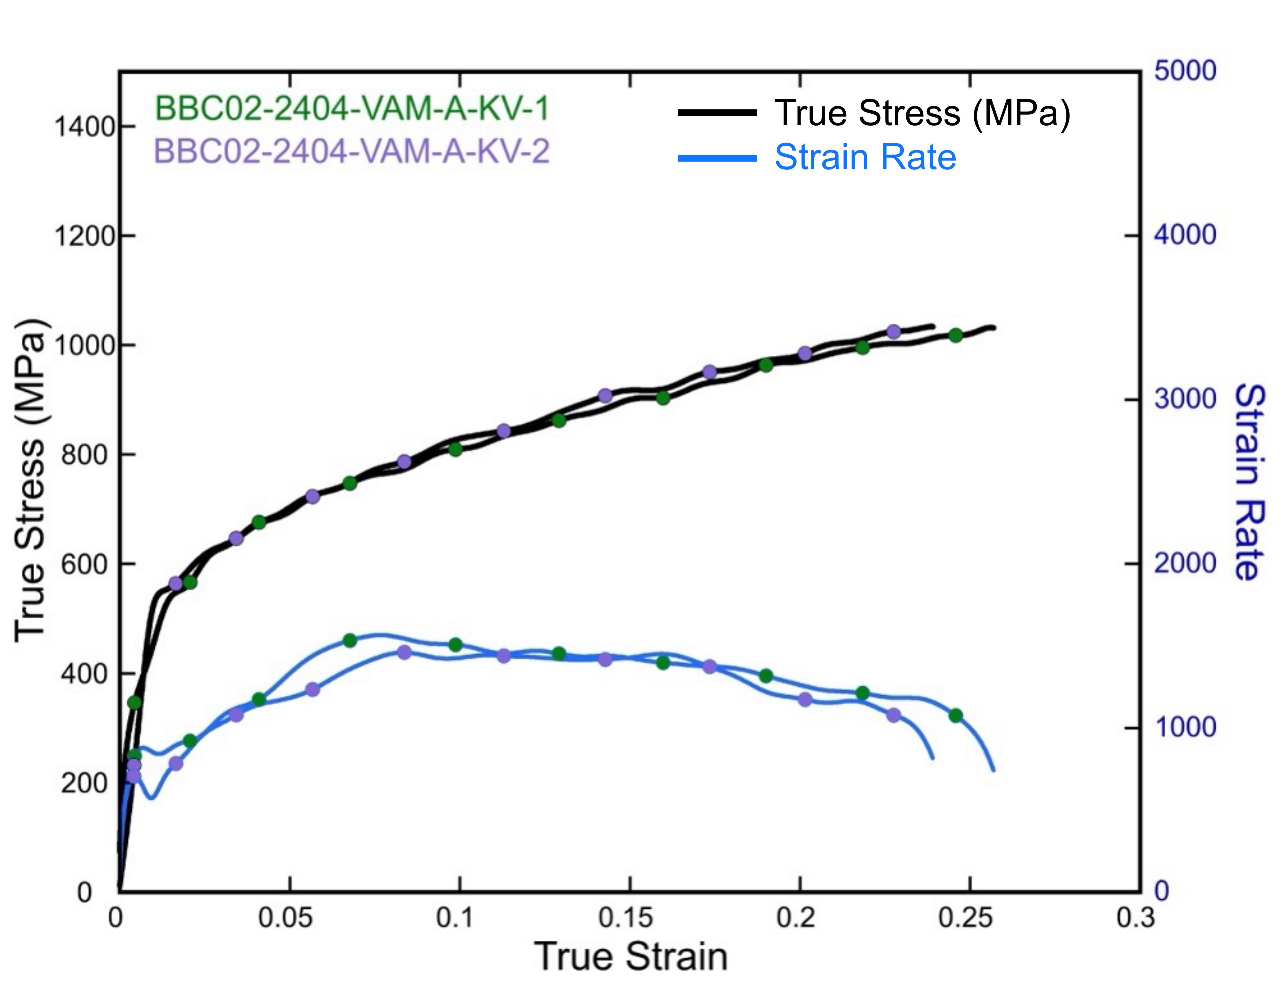
\includegraphics[width=0.9\columnwidth]{Figures/SPHB2.pdf}
    \caption{Dynamic true stress–strain responses (black) and corresponding strain rate as a function of strain (blue) for two HEA samples tested at 1500\,s$^{-1}$.}
    \label{fig:shpb_signals}
\end{figure}


\subsection{Depth of Penetration Simulation}

\emph{Viscoplasticity Constitutive Model Implementation:} We modeled the ballistic impact response using the Cowper-Symonds (CS) viscoplasticity framework to capture strain rate sensitivity under dynamic loading. The CS model provides a description of the flow stress evolution as a function of plastic strain rate through a multiplicative enhancement factor applied to the quasi-static flow strength. The constitutive relationship is expressed as:

\begin{equation}
\sigma_f = \sigma_{qs}^f \left(1 + \left(\frac{\dot{\varepsilon}_p}{D}\right)^{1/M}\right)
\end{equation}

where $\sigma_{qs}^f$ represents the quasi-static flow strength that evolves with accumulated plastic strain due to work hardening mechanisms, $\dot{\varepsilon}_p$ denotes the effective plastic strain rate, $D = 10^6 \text{ s}^{-1}$ serves as a material-dependent constant multiplier, and $M$ constitutes the strain rate sensitivity exponent within the CS formulation. This formulation captures dynamic strengthening at elevated loading rates, where dislocation motion becomes increasingly constrained.

In the Cowper--Symonds form, $D$ and $M$ are mathematically coupled: for a given pair of quasi-static and dynamic flow-stress measurements, a continuum of $(D, M)$ combinations can reproduce the data with comparable fidelity. With one SHPB curve and one quasi-static curve per alloy, joint identification of both parameters is underdetermined. We resolve this by fixing $D = 10^{6}\ \text{s}^{-1}$ uniformly across all alloys and calibrating $M$ per alloy by RMSE minimization against the experimental QS+SHPB data (Eq.~\ref{eq:rmse}. This convention isolates the alloy-to-alloy variation in a single rate-sensitivity parameter, allows direct comparison of $M$ across the composition set on a common basis.

\emph{Rate Sensitivity Parameter Identification:} The strain rate sensitivity parameter $M$ for each high entropy alloy composition was determined through a systematic calibration procedure based on experimental data obtained from quasistatic uniaxial tension tests and dynamic SHPB compression experiments conducted at strain rates ranging from $10^{-3} \text{ s}^{-1}$ to $10^4 \text{ s}^{-1}$. The parameter identification process used a nonlinear least-squares optimization algorithm to minimize the root mean squared error (RMSE) between the CS model predictions and experimental true stress measurements:

\begin{equation}
\text{RMSE} = \sqrt{\frac{1}{N}\sum_{i=1}^{N}\left(\sigma_{pred,i}^f - \sigma_{obs,i}^f\right)^2}
\label{eq:rmse}
\end{equation}

where $N$ represents the total number of discrete data points in the experimental stress-strain response, $\sigma_{pred,i}^f$ denotes the model-predicted flow stress at the $i$-th data point, and $\sigma_{obs,i}^f$ corresponds to the experimentally observed true stress value. The optimization procedure was implemented under isothermal conditions to isolate the strain rate effects from thermal softening mechanisms. The calibrated rate sensitivity exponents for the investigated high entropy alloy compositions ranged between 2 and 7, consistent with the expected strain rate sensitivity behavior of face-centered cubic polycrystalline materials.

\emph{Finite Element Ballistic Impact Simulation:} We implemented the calibrated material parameters into a user-defined material subroutine (UMAT) within the ABAQUS/Explicit finite element framework to simulate the ballistic impact response. The computational model used a two-dimensional axisymmetric formulation to simulate the normal impact of a rigid spherical projectile onto a cylindrical target of the candidate alloy. The target geometry consisted of a cylinder with radius $r_t = 34$ mm and thickness $t = 17$ mm, while the projectile was modeled as a rigid sphere with diameter $d_p = 10$ mm impacting at a velocity of $V_0 = 500$ m/s.

The finite element discretization used explicit, linear, axisymmetric stress elements (CAX4R) with a characteristic mesh size of 0.8 mm, resulting in a computational domain of 42 $\times$ 21 elements in the radial and axial directions, respectively. The target material properties included an elastic modulus $E_t = 200$ GPa, Poisson's ratio $\nu_t = 0.3$, and density $\rho_t = 7.85 \times 10^{-9}$ ton/mm³. Mesh distortion controls were implemented using default ABAQUS settings. The elastic constants and density are held fixed across all the alloys. This reflects both the available characterization data and a deliberate scoping choice. The quasi-static tension and SHPB experiments resolve only the plastic flow response of each alloy; elastic moduli and densities were not independently measured for individual compositions, so representative steel-class values ($E_t = 200$ GPa, $\rho_t = 7.85 \times 10^{-9}$ ton/mm$^3$) were used uniformly. For Ni-stabilized FCC HEAs representative of the type studied here, Young's modulus and Poisson's ratio are expected to vary by less than $\sim$10\% across compositions and to contribute negligibly to penetration response, which is dominated by plastic dissipation at 500 m/s. 


\emph{Depth of Penetration Quantification:} The ballistic performance of each alloy composition was quantified through the depth of penetration (DoP), defined as the maximum axial displacement of the projectile centroid into the target at the instant when the projectile velocity approaches zero. DoP serves as the primary response variable for correlating material properties with impact performance. All alloys across the three optimization iterations were evaluated under identical loading conditions using their individually calibrated viscoplastic constitutive models.


\subsection{Computational Design Framework}

The computational component of BRAVE linked thermodynamic screening, physics-informed surrogate modeling, feasibility classification, multi-objective acquisition, and diversity-aware batch selection into one loop. In each iteration, experimentally verified FCC alloys provided objective data for surrogate updates, while infeasible alloys contributed only their phase labels to the feasibility model. A more detailed end-to-end workflow diagram is provided in the \textbf{SI}.

\subsubsection{Surrogate Models and Objective Representation}

We used Gaussian process surrogate models because they provide both property predictions and uncertainty estimates, which are needed for Bayesian optimization. The surrogates were initialized with informative priors rather than zero-mean priors, using the Varvenne--Luque--Curtin solid solution strengthening model together with prior campaign data to provide a physics-grounded starting point before substantial new data were collected. Detailed mathematical expressions for the GP posterior and prior construction are provided in the Appendix.

The optimization targeted the five objectives defined in Section~2.3. Four objectives (YS, UTS/YS, strain at UTS, and $H_\text{dyn}/H_\text{qs}$) were obtained experimentally, while DoP was computed from constitutive calibration and FEM simulation using data acquired in the same iteration. Because EHVI is implemented in minimization form, the four desirable-to-maximize objectives were sign-inverted before surrogate modeling and hypervolume calculation, while DoP remained in its original minimization form.

\subsubsection{Acquisition, Fusion, and Batch Selection}

Candidate ranking was based on Expected Hypervolume Improvement (EHVI), which favors alloys expected to improve the current Pareto front while still exploring uncertain regions. Where multiple computational estimates contributed to the same target, their predictions were fused through a reification-based multi-source model so that the acquisition function operated on a single posterior distribution for each objective. To reduce sensitivity to any one kernel hyperparameter setting in the low-data regime, we used an ensemble of Gaussian processes with different length-scale assumptions and then applied $k$-medoids clustering to select a diverse experimental batch. Mathematical details for EHVI, reification, and the batch ensemble strategy are provided in the Appendix.

\subsubsection{Constraint-Aware Acquisition with Learned Feasibility}

Phase stability constraints were enforced initially through CALPHAD screening, but deterministic rejection alone is too rigid near the FCC phase boundary. We therefore trained a Gaussian process classifier (GPC) on experimentally verified phase outcomes to estimate a continuous feasibility probability, $P_\text{feas}(\mathbf{x})$, for each candidate composition. This allowed the optimizer to distinguish compositions that were confidently infeasible from those that were merely uncertain.

To assess how robust CALPHAD-predicted FCC stability is to small local composition changes, we performed a perturbation analysis on candidate alloys that satisfied FCC $\geq 0.99$. Of the 1,154,207 perturbed compositions evaluated, 903,326 (78.3\%) retained FCC $\geq 0.99$. We therefore interpreted a feasibility probability near 0.8 as corresponding to a composition that is locally robust to small perturbations, which motivated the acquisition threshold $P_\text{feas}(\mathbf{x}) \geq 0.8$. Details are provided in the \textbf{SI}.

Candidates that passed the initial CALPHAD filter were assigned $P_\text{feas} = 1$. Candidates rejected by CALPHAD but predicted by the GPC to satisfy $P_\text{feas}(\mathbf{x}) \geq 0.8$ were reintroduced into the search space, but their acquisition value was penalized according to feasibility risk:
\begin{equation}
    \textrm{EHVI}(\mathbf{x})_{\textrm{constraint-aware}} = \textrm{EHVI}(\mathbf{x}) \times P_{\textrm{feas}}(\mathbf{x})
\end{equation}
This feasibility-weighted acquisition suppressed high-risk candidates whose apparent promise was driven mainly by uncertainty, while still allowing near-boundary alloys to be selected when their predicted performance was sufficiently strong. As new alloys were synthesized and phase-verified, the GPC was retrained so that the feasibility boundary improved over successive iterations. Manufacturing failures were not modeled by this classifier; it addressed phase-outcome feasibility only.

\subsubsection{Summary of the BRAVE Campaign Algorithm}

\autoref{fig:brave_architecture} illustrates the data flow within a single iteration of the BRAVE campaign. The bifurcation at phase verification was the defining structural feature: feasible alloys proceeded through full characterization and fed objective data into the GP surrogates, while infeasible alloys contributed only their phase outcome to the GPC feasibility classifier. Both paths converged at the acquisition step, where EHVI was weighted by the learned feasibility probability. Algorithm~\ref{alg:brave} formalizes this workflow.

Algorithm~\ref{alg:brave} consolidates the full BRAVE campaign workflow, from design space initialization through iterative closed-loop optimization. Infeasible alloys (line~9) contribute to the feasibility classifier but not to surrogate model training, capturing the asymmetry between failed and successful experiments that motivates the risk-aware acquisition strategy. The DoP objective (lines~16--18) is computed within each iteration from experimentally calibrated constitutive models, creating the simulation-in-the-loop architecture described in Section~1.

\begin{algorithm}[!htbp]
\caption{BRAVE: Bayesian Risk-Aware Alloy Discovery and Exploration}\label{alg:brave}
\begin{algorithmic}[1]
\Statex \textbf{Input:} 8-element composition grid, CALPHAD database, batch size $B = 16$
\Statex
\Statex \textit{// Initialization}
\State Apply compositional bounds $\rightarrow$ 1,504,938 candidates
\State CALPHAD screen (TCHEA6, FCC $\geq 0.99$ at 700$^\circ$C) $\rightarrow$ 26,621 feasible
\State Partition feasible space into 37 chemical subsystems
\State Retain subsystem labels for feasible candidates
\State $k$-medoids clustering $\rightarrow$ 1,000 representative alloys
\State Diversity-aware down-selection $\rightarrow$ $B_0 = 16$ initial candidates
\Statex
\Statex \textit{// Mid-campaign update (from iteration BBB onward)}
\State Augment feasibility screening using TCHEA7 (700$^\circ$C and 950$^\circ$C)
\State Update feasible design space
\Statex
\Statex \textit{// Iterative closed-loop optimization}
\For{iteration $t = 0, 1, 2$}
    \State Synthesize $B_t$ alloys via vacuum arc melting
    \State Verify phase purity (XRD): classify each alloy as \textit{feasible} or \textit{infeasible}
    \State Update GPC feasibility classifier with new phase outcomes
    \For{each \textit{feasible} alloy}
        \State Characterize: tensile $\rightarrow$ YS, UTS/YS, strain at UTS
        \State Characterize: NI + HSRNI + SHPB $\rightarrow$ $H_\text{dyn}/H_\text{qs}$
        \State Calibrate Cowper--Symonds model from tensile + SHPB data
        \State Simulate depth of penetration (DoP) via FEM with calibrated model
    \EndFor
    \State Update GP surrogates with new objective measurements (feasible alloys only)
    \State Fuse multi-source predictions via reification
    \For{each of $n$ random length-scale configurations}
        \State Build GP ensemble member
        \State Compute $\textrm{EHVI}(\mathbf{x}) \times P_\text{feas}(\mathbf{x})$ for all remaining candidates
    \EndFor
    \State $k$-medoids select $B_{t+1}$ from top-ranked candidates
\EndFor
\Statex
\Statex \textbf{Output:} Pareto-optimal alloys, trained surrogates, feasibility classifier
\end{algorithmic}
\end{algorithm}


\begin{figure*}[t]
    \centering
    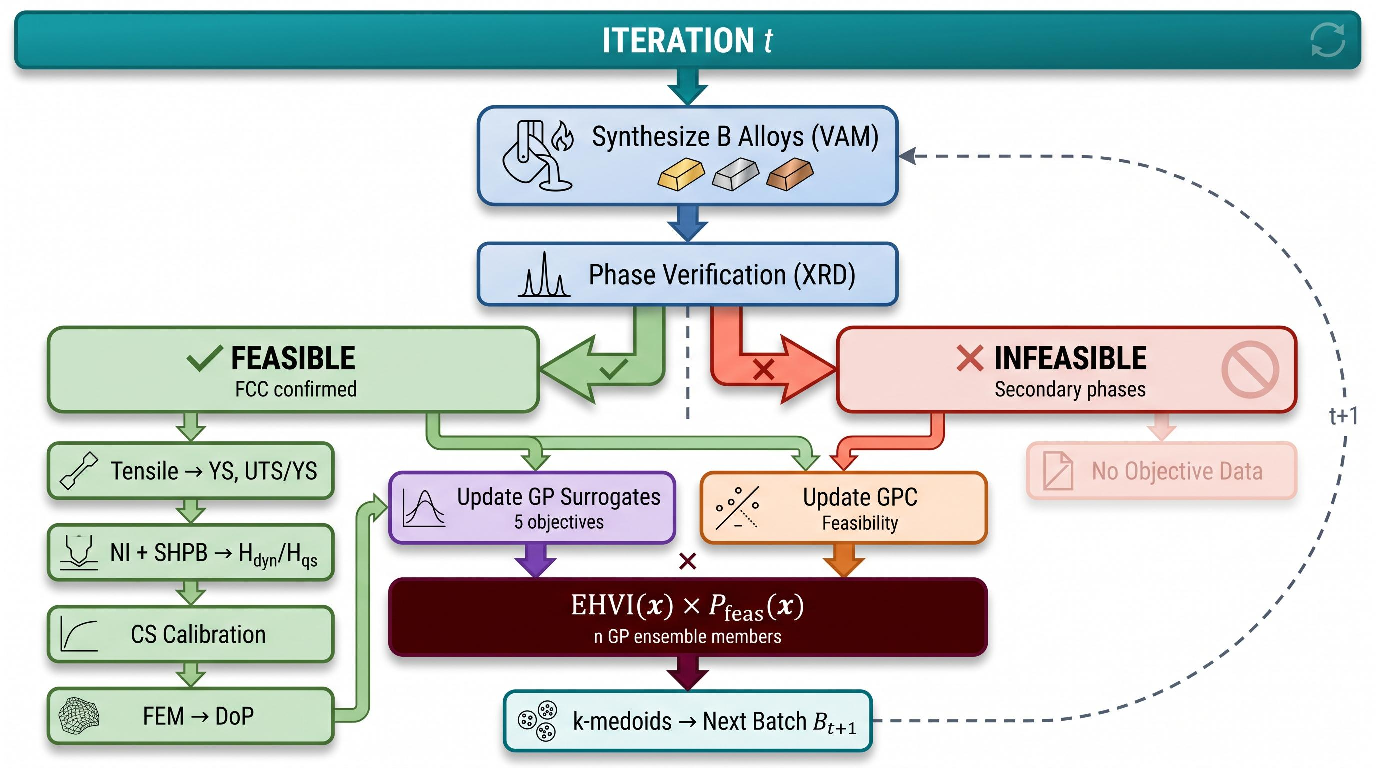
\includegraphics[width=0.9\textwidth]{Figures/brave_architecture.pdf}
    \caption{Data flow architecture for one iteration of the BRAVE campaign. Phase verification (XRD) classifies each synthesized alloy as feasible or infeasible, creating two parallel update paths: feasible alloys provide objective measurements for GP surrogate training, while all phase outcomes (feasible and infeasible) update the GPC feasibility classifier. The paths converge at the acquisition step, where EHVI is scaled by the feasibility probability $P_\text{feas}(\mathbf{x})$ to penalize high-risk candidates. k-medoids clustering selects the next batch from the top-ranked candidates.}
    \label{fig:brave_architecture}
\end{figure*}


The campaign ran for three iterations (48 alloys total). This budget was set by experimental throughput---vacuum arc melting, thermomechanical processing, and multi-technique characterization limit the number of alloys that can be completed per cycle---rather than by a convergence criterion.


\subsection{Data Management and Overall Workflow}

Data management in this study follows a method-centric architecture with IGSN (International Generic Sample Number) registration for all physical samples. Details of the data architecture, folder structure, IGSN metadata schema, FAIR compliance, and a more detailed end-to-end workflow diagram are provided in the \textbf{SI}.
